\section{Antenna Design 2 -- Triangle-Feed Antenna}
\label{sec:techsol_triang}

\begin{figure}[htbp]
    \begin{subfigure}[b]{0.49\linewidth}
        \centering
        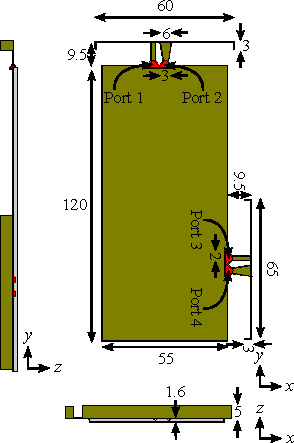
\includegraphics{img/tech_sol/trianglefeed/technical}
        \caption{Technical drawing. Unit: mm.}
        \label{fig:ant2technical}
    \end{subfigure}
    \hfill
    \begin{subfigure}[b]{0.49\linewidth}
        \centering
        \includegraphics{img/tech_sol/schematic_tuning_1}\\[1cm]
        \footnotesize
        \begin{tabular}{|l|l|l|l|}
            \hline
            & $C_1$ & $L_1$ & $C_2$ \\
            \hline
            Top antenna & \SI{3.45}{pF} & \SI{7.89}{nH} & $[0.3,2.9]\,$pF\\
            Side antenna & \SI{2.42}{pF} & \SI{5.69}{nH} & $[0.3,2.9]\,$pF\\
            \hline
        \end{tabular}
        \caption{Tuning/matching circuit.}
        \label{fig:ant2schematic}
    \end{subfigure}
    \caption{Technical drawing and tuning circuit for the antenna.  The antennas are built on FR-4 board using \SI{35}{\micro\meter} copper. There is a matching circuit as shown for each of the two feeds.}
    \label{fig:ant2techschem}
\end{figure}

The antenna is shown in Figure~\ref{fig:ant2techschem}. The two antennas each consist of a triangle-feed printed on FR-4 and the main element following the edge of this FR-4 block.

% What makes it radiate at 900, 1800, and 2400?
The low-band element consists of a CCE (Capacitively Coupled Element) antenna which is inherently non-resonant \cite{valkonen2013inherently,ilvonen2014design}. The resonance of this type of antenna is dependent on the matching circuit. For this design, the matching is performed by $C_1$ and $L_1$ to resonate at \SI{960}{MHz} and $C_2$ is used to tune the resonance frequency down to \SI{700}{MHz}.

The triangular feed creates two new resonances in the mid-band (around \SI{1800}{MHz}) and the high-band (around \SI{2400}{MHz}). Looking at the top-antenna, the right-hand side from the feed line resonates at around \SI{1800}{MHz} and the left-hand side resonates at around \SI{2400}{MHz}. By determining the $x$-position of the triangle-feed, these two resonances can either be separated or joined, making it possible to cover all the required high LTE bands. The surface currents, illustrating how the structure resonates after matching, is shown in Figure~\ref{fig:ant2surfaces}.

\begin{figure}[htbp]
    \centering
    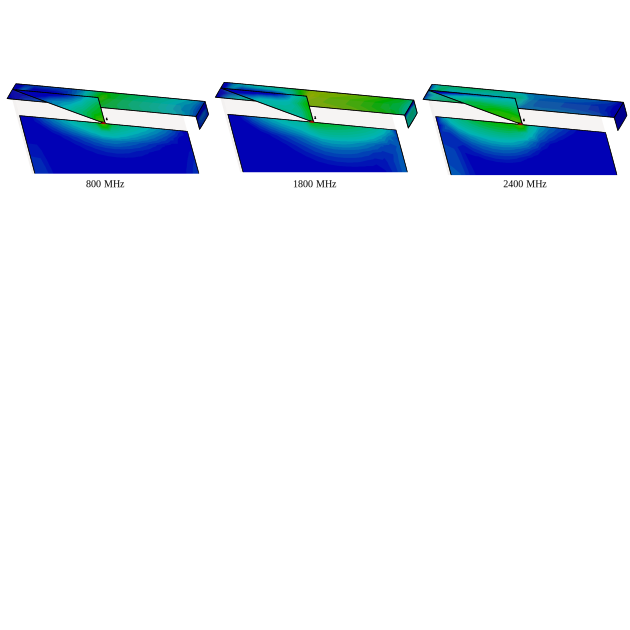
\includegraphics{img/tech_sol/trianglefeed/surface_currents}
    \caption{Surface currents around each resonance with $C_2=\SI{0.3}{pF}$.}
    \label{fig:ant2surfaces}
\end{figure}

\begin{figure}[htbp]
    \centering
    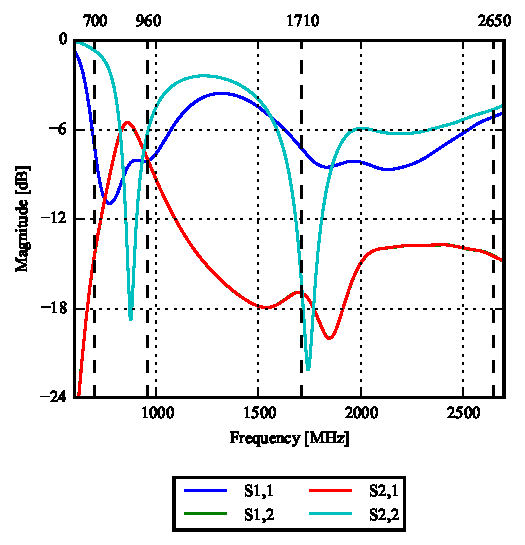
\includegraphics{img/tech_sol/trianglefeed/sparams}
    \caption{S-parameters with $C_2=\SI{0.3}{pF}$ for both antennas.}
    \label{fig:ant2sparams}
\end{figure}

The S-parameters for both antennas are shown in Figure~\ref{fig:ant2sparams} with the tuning capacitors at their minimum values, \SI{0.3}{pF}. At this position, the highest end of the low band, around \SI{960}{MHz}, is covered. It is seen that the top-antenna (port 1) covers the whole lower band whereas the side-antenna only covers around half of the band and must be tuned to cover the whole band. The high band is almost covered at this capacitor setting for both antennas.

The tuned S-parameters are shown in Figure~\ref{fig:ant2sweeps}. Here is seen that the whole lower band can be covered by the side antenna ($S_{22}$) and that the whole high band is covered at $C_2 = \SI{0.7}{pF}$ to \SI{0.9}{pF} for the top- and side-antenna respectively. It is noted that all three resonances are moved when $C_2$ is altered.

% Sweep description
It is seen that the isolation at low frequencies is only around \SI{5}{dB}. This may cause problems when using the antennas for MIMO operation. The bad isolation may be caused by the way the CCE antenna resonates. The CCE antenna couples to the chassis an uses this as a resonator \cite{ilvonen2014design}. This may cause high correlation when both antennas couple to the chassis.

This design provides high bandwidth, covering all desired bands for both antennas. However, the isolation between the two antennas is not the best. Additionally, building the antenna on lossy FR-4 may prove to decrease the efficiency bandwidth compared to an antenna with a less lossy isolator.

\begin{table}[htbp]
    \centering
    \begin{tabular}{|l|l|r|r|r|}
        \hline
        Antenna & Band & Start [MHz] & Stop [MHz] & Bandwidth [MHz] \\
        \hline
        Top     & Low  & 688         & 1073       & 385 \\
        Side    & Low  & 824         & 962        & 138 \\
        \hline
        Top     & High & 1577        & 2637       & 1060 \\
        Side    & High & 1535        & 2654       & 1119 \\
        \hline
    \end{tabular}
    \caption{Maximum bandwidth obtained in the low and high band for the top and the side antenna, respectively.}
    \label{tab:bw_sol2}
\end{table}

% Bandwidth
The bandwidth in the high and low band for each antenna is shown in Table~\ref{tab:bw_sol2}. It is clear that both antennas fulfill the requirements of tunable impedance bandwidth seen in the requirement specification, Section~\ref{cha:reqspec}.

\begin{figure}[htbp]
    \centering
    \begin{subfigure}{0.49\linewidth}
        \centering
        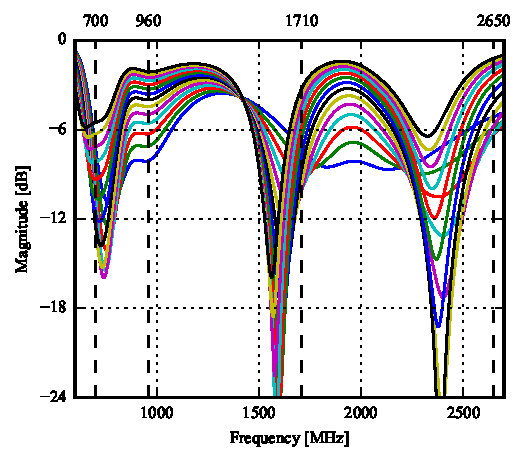
\includegraphics{img/tech_sol/trianglefeed/Csh1s11.pdf}
        \caption{$S_{11}$, sweeping $C_1$ and fixing $C_2$.}
    \end{subfigure}
    \hfill
    \begin{subfigure}{0.49\linewidth}
        \centering
        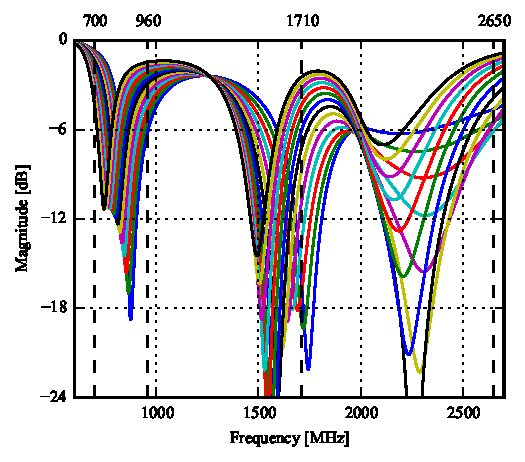
\includegraphics{img/tech_sol/trianglefeed/Csh2s22.pdf}
        \caption{$S_{22}$, sweeping $C_2$ and fixing $C_1$.}
    \end{subfigure}
    \vspace*{1em}
    \begin{subfigure}{0.49\linewidth}
        \centering
        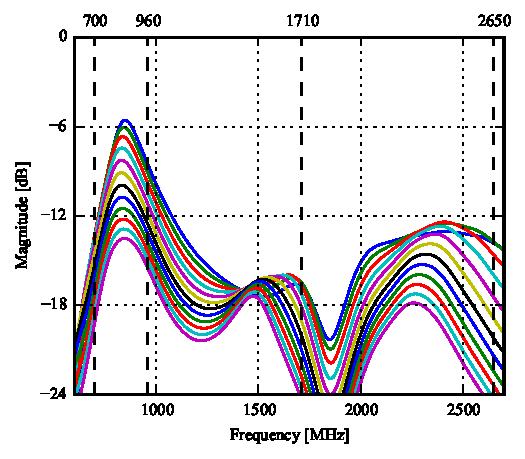
\includegraphics{img/tech_sol/trianglefeed/Csh1s21.pdf}
        \caption{$S_{21}$, sweeping $C_1$ and fixing $C_2$.}
    \end{subfigure}
    \hfill
    \begin{subfigure}{0.49\linewidth}
        \centering
        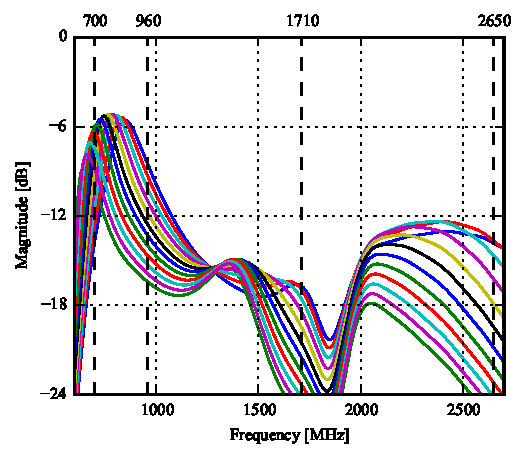
\includegraphics{img/tech_sol/trianglefeed/Csh2s21.pdf}
        \caption{$S_{21}$, sweeping $C_2$ and fixing $C_1$.}
    \end{subfigure}
    \caption{Parameter sweeps when tuning the shunt capacitor of each antenna, $C_{1}$ and $C_{2}$ for port 1 and 2, respectively. Port 1 is the top antenna and port 2 is the side antenna.}
    \label{fig:ant2sweeps}
\end{figure}

% Correlation
\begin{figure}[htbp]
    \centering
    \begin{subfigure}{0.49\linewidth}
        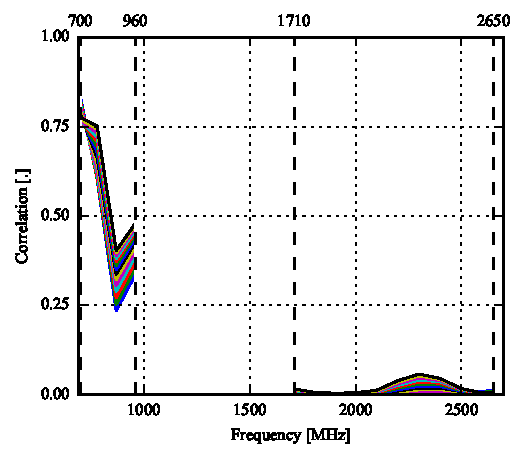
\includegraphics{img/tech_sol/trianglefeed/corr/correlation_Csh1-sweep}
        \caption{Sweeping $C_1$ and fixing $C_2$.}
    \end{subfigure}
    \hfill
    \begin{subfigure}{0.49\linewidth}
        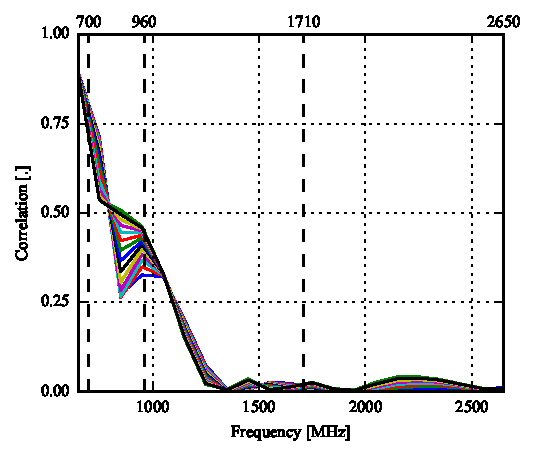
\includegraphics{img/tech_sol/trianglefeed/corr/correlation_Csh2-sweep}
        \caption{Sweeping $C_2$ and fixing $C_1$.}
    \end{subfigure}
    \caption{Correlation between antennas then sweeping tuning capacitors. Here, $C_1$ and $C_2$ are the tuning capacitor for the top and side antenna, respectively.}
    \label{fig:corr_sol2}
\end{figure}
The correlation between the top an side antennas are shown in Figure~\ref{fig:corr_sol2} when sweeping the tuning capacitors. It is seen that the correlation in the high band is very low while the correlation in the low band is not the best. This may be caused by the fact that both antennas are coupling to the ground plane to radiate. A solution might be to use a different type of antenna for the side than for the top.

% Efficiency
\begin{figure}[htbp]
    \centering
    \begin{subfigure}{0.49\linewidth}
        \centering
        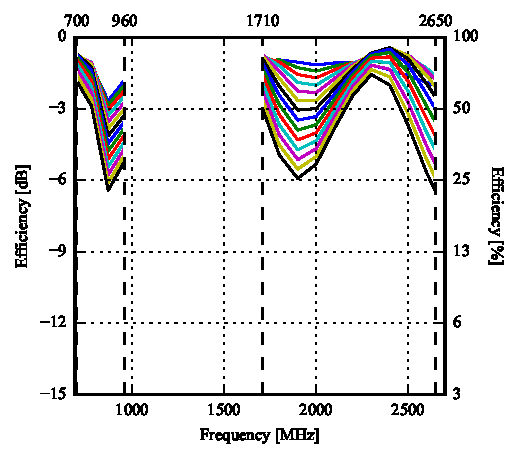
\includegraphics{img/tech_sol/trianglefeed/efficiency-ac1-csh1.pdf}
        \caption{Top antenna. Sweeping $C_1$, fixing $C_2$.}
    \end{subfigure}
    \hfill
    \begin{subfigure}{0.49\linewidth}
        \centering
        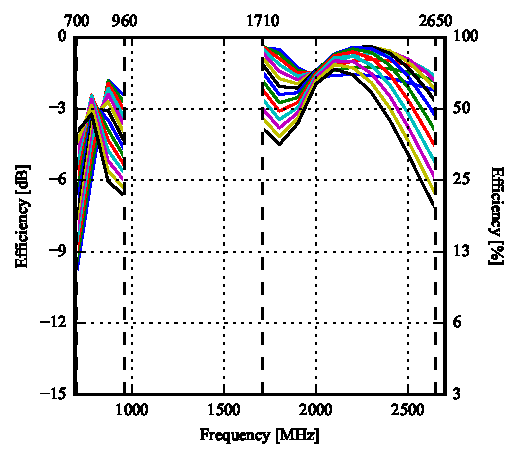
\includegraphics{img/tech_sol/trianglefeed/efficiency-ac2-csh2.pdf}
        \caption{Side antenna. Sweeping $C_2$, fixing $C_1$.}
    \end{subfigure}
    \caption{Efficiency for each antenna when sweeping the tuning capacitors. Here, $C_1$ and $C_2$ are the tuning capacitor for the top and side antenna, respectively.}
    \label{fig:eff_sol2}
\end{figure}
The total system efficiency (i.e.\ including mismatch loss) is shown for a sweep of capacitance values in Figure~\ref{fig:eff_sol2}. It is seen that, for the lowest capacitance setting, the top antenna has a total efficiency greater than \SI{-3}{dB}. The side antenna has a total efficiency greater than \SI{-3}{dB} in the high band for its low capacitance settings. In the low band, the antenna can be tuned to cover the whole band at a total efficiency above \SI{-4}{dB}.
